\documentclass[tikz,border=6pt]{standalone}
\usepackage{pgfplots}
\pgfplotsset{compat=1.18}
\usepgfplotslibrary{fillbetween}
\usepackage{amsmath}
\usetikzlibrary{arrows.meta,fit,positioning}

\begin{document}
	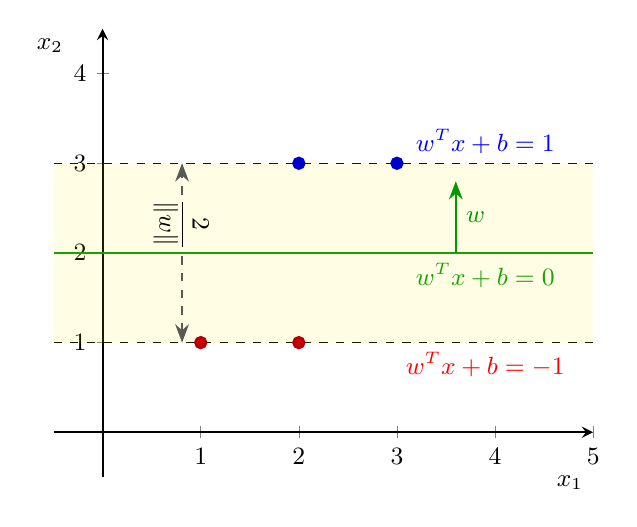
\begin{tikzpicture}[every node/.style={font=\small},>=Stealth]
		\begin{axis}[
			scale=1.0,
			xmin=-0.5, xmax=5,
			ymin=-0.5, ymax=4.5,
			axis lines=middle,
			xlabel={$x_{1}$},
			ylabel={$x_{2}$},
			xlabel style={at={(axis description cs:1,-0.05)}},
			ylabel style={at={(axis description cs:-0.05,1)}},
			thick
			]
			% Data points
			\addplot+[only marks, mark=*, mark size=2pt, color=blue!80!black]
			coordinates { (2,3) (3,3) };
			\addplot+[only marks, mark=*, mark size=2pt, color=red!70!black]
			coordinates { (1,1) (2,1) };
			
			% Decision boundary and margins
			\addplot[thick,green!60!black] coordinates {(-0.5, 2)(5, 2)}
			node[pos=0.8, below, green!60!black,font=\small] {$w^{T}x+b=0$};
			\addplot[dashed,thin,black] coordinates {(-0.5, 3)(5, 3)}
			node[pos=0.8, above, blue,font=\small] {$w^{T}x+b=1$};
			\addplot[dashed,thin,black] coordinates {(-0.5, 1)(5, 1)}
			node[pos=0.8, below, red,font=\small] {$w^{T}x+b=-1$};
			\fill[yellow,opacity=0.1] (-0.5,1) rectangle (5,3);
			
			% Normal vector w
			\draw[->,thick,green!60!black] (3.6,2) -- (3.6,2.8)
			node[pos=0.5,right,font=\small] {$w$};
			
			% Margin indication with a gap (breakable dashed line)
			\draw[<-,thick,dashed,gray!70!black]
			(0.81,1) -- (0.81,2.02);
			\draw[->,thick,dashed,gray!70!black]
			(0.81,2.65) -- (0.81,3);
			\node[rotate=-90,font=\small] at (0.8,2.32) {$\displaystyle \frac{2}{\|w\|}$};
		\end{axis}
	\end{tikzpicture}
\end{document}
